\documentclass[12pt]{article}

% Packages
\usepackage[utf8]{inputenc} % allow utf-8 input
\usepackage[T1]{fontenc}    % use 8-bit T1 fonts
\usepackage{geometry}       % to change the page dimensions
\usepackage{graphicx}       % support the \includegraphics command and options
\usepackage{amsmath}        % for better mathematical formulas
\usepackage{amsfonts}       % for mathematical fonts
\usepackage{amssymb}        % for mathematical symbols
\usepackage{hyperref}       % for hyperlinks
\usepackage{lipsum}         % for generating filler text
\usepackage{float}          % for better figure placement
\usepackage{natbib}         % for better citations
\usepackage{pdfpages}       % for including pdfs
\bibliographystyle{unsrtnat}

% Page geometry
\geometry{a4paper, margin=1in}

\begin{document}

%Title Page
\begin{titlepage}
    \centering
    \vspace*{5cm}

    \Large
    \textbf{Swarm Robotics: Exploration and Mapping in Simulated testing Environments}

    \vspace{1cm}

    Charlie Anthony [CandNo: 246537]\\
    Supervisor: Dr Chris Johnson



    \vfill

    \vspace{1cm}

    \small
    Interim report\\
    Computer Science and Artificial Intelligence BSc

    
\includegraphics[width=0.3\linewidth]{sussex_logo.jpg}


    \small
    Department of Informatics and Engineering\\
    University of Sussex\\
    November 2023
\end{titlepage}

%Table of Contents
\tableofcontents
\newpage

%Introduction
\section{Introduction}
Swarms exist everywhere in life. Nearly all organisms exhibit some form of swarming behaviours within their
communities. Starlings display impressive organisational behaviour, positioning themselves with respect to the
movement of their neighbours \cite{starling_swarm}. Humans show swarm behaviours when moving in crowds, for example, moving around sports
venues or exiting buildings in emergencies. No matter how hard you look, regardless if the context, swarms are
typically present.\\
These behaviours can also be artificially created in robotics \cite{intro_to_swarm}. Within the realm of computing, parallelising
processes is breaking barrier after barrier - swarm robotics brings the same benefits. Being able to divide and
conquer a problem has the ability to massively increase the rate of work by employing multiple robots. Therefore, it
would be wasteful not to properly dedicate the time which this discipline deserves.\\
For my project, I am going to try and reproduce some of these behaviours artificially. I will start by simulating robotic
agents in a 2D environment. The agents will be placed within close proximity inside a simulated environment and then allowed
to explore and combine their findings; ultimately creating a visualization map of its environment. The agents will need to
both navigate the environment and avoid collisions, whilst creating an internal representation of its surroundings. The
best-case scenario for the agents within the swarm is to be fully independent; creating a decentralized system.\\
I will initially explore this problem by creating SLAM simulations, and then attempting to apply similar techniques
to a centralised system. These initial simulations will employ techniques such as graph-based SLAM, random walks and other elements of
swarm behaviours in order to create a base-line representation of the environment. This project will also have the flexibility to
potentially implement physical robots, given time permits.\\

%Professional and Ethical Considerations
\section{Professional and Ethical Considerations}
My project maintains compliance towards all ethical considerations, as there is minimal external involvement from
humans. The majority of my project will be carried out in simulation, therefore no ethical approval is required. Should
my project progress to physically implementing agents, considerations such as safety around the robots, will be considered.
All tests will be carried out in an environment where people cannot be hit, therefore mitigating any trip hazards.\\

To ensure all elements of the BCS code of conduct are met, I have summarised each section and how I meet certain criteria. \\
\subsection{Public Interest}
As mentioned previously, my project has due regard for public health, as there is minimal external involvement from humans.
Furthermore, no major privacy, security or wellbeing considerations are required due to the nature of this project. Third parties
will be respected throughout the project with consistent citations and there will be no discrimination against anybody involved.
Finally, I will promote equal access to the benefits of IT by open-sourcing my research once I have graduated. This will be accessible
on my Github profile: \href{https://github.com/CharlieAnthony/}{https://github.com/CharlieAnthony/} \\
\subsection{Professional Competence and Integrity}
My project is within my professional competence, as it significantly relies upon knowledge obtained from modules such as "Acquired
Intelligence and Adaptive Behaviour" and "Fundamentals of Machine Learning." Furthermore, I will develop my professional knowledge,
skills and competence through communicating with my supervisor and ensuring all relevant gaps in knowledge are explored through
reading extensively. As part of my background reading, I have made myself familiar with the BCS code of conduct and surrounding
legistlation. I will comply with this throughout when carrying out my professional responsibilities. There will also
be no unethical inducements offered or accepted throughout the project. \\
\subsection{Duty to Relevant Authority}
As the relevant authority will be the University of Sussex, I will comply with all relevant codes of conduct and legislation. I
will exercise my professional judgement at all times, including avoidance of any situation that may give rise to a conflict of
interest between myself and the university. I will also make it my responsibility to ensure all colleagues work is properly
referenced in a bibliography at the end of my dissertation. \\
\subsection{Duty to the Profession}
Finally, I accept my duty to uphold the reputation of the profession. I will work to the best of my ability to ensure my project
is complete to the highest possible standard. As mentioned previously, I will seek to improve professional standards through
communication with my supervisor. This dissertation will be written with integrity and respect towards all members of BCS and colleagues
of the profession. \\


%Related Work
\section{Related Work}
\subsection{SLAM}

\begin{figure}[h]
    \centering
    \begin{minipage}{0.45\textwidth}
        \centering
        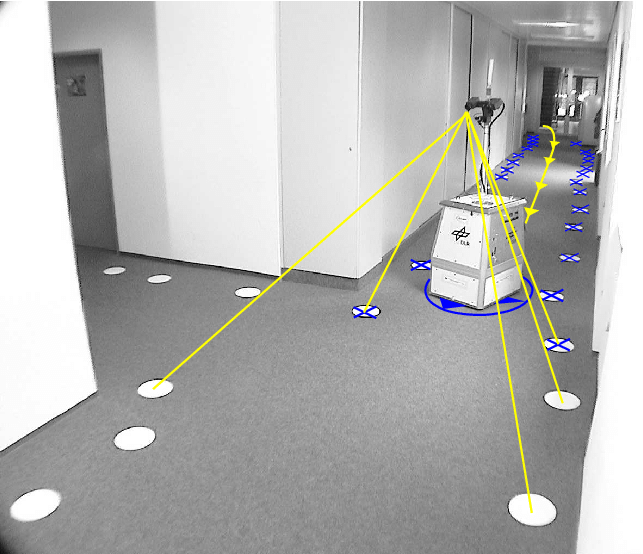
\includegraphics[width=\linewidth]{SLAM_agent} % First image
        \caption[Short caption]{A visual representation of a robot scanning its environment \cite{SLAM_overview}}
        \label{fig:SLAM_agent}
    \end{minipage}\hfill
    \begin{minipage}{0.45\textwidth}
        \centering
        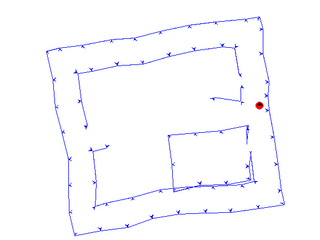
\includegraphics[width=\linewidth]{SLAM_map} % Second image
        \caption[Short caption]{The map (after loop closure) produced by the robot's SLAM algorithm of its environment \cite{SLAM_overview}}
        \label{fig:SLAM_map}
    \end{minipage}
\end{figure}

SLAM (Simultaneous Localisation and Mapping) is a technique used in robotics to create a map of an unknown environment \cite{SLAM_overview}.
It is an important area of research in robotics as it is heavily used in autonomous vehicles, drones and vacuum cleaners;
allowing agents to understand and navigate their environment effectively. Figure \ref{fig:SLAM_agent} shows an example of a
robot scanning its environment, with the sensors visually added to the image.\\
SLAM can be broken down into two sub-problems: localisation and mapping. Localisation is the process of determining the
location of a robot in its environment, whilst mapping is the process of constructing a map of the environment. The maps
are constructed using data collected from sensors, such as cameras and laser scanners; Figure \ref{fig:SLAM_map} shows this.
A lot of existing work in SLAM is based on single robot applications, however, there is a growing interest in multi-agent
SLAM. One of the greatest challenges in SLAM is crossing the simulation to reality gap, as in the real world, sensor
readings are noisy and environments are dynamic, which increases the complexity of the problem.

\subsection{Graph-based SLAM}
Graph-based SLAM is a technique used to create a map of an environment, by using a graph to represent the environment. It
works by having a robot move around its environment, whilst taking measurements of its surroundings. These measurements
are usually received by a sensor, such as a camera or laser scanner. The robot then uses these measurements to create a
plot of where objects may be, by combining the measurements from sensors with its memory of the route it has taken. This
technique is used in many applications, both in research and in the real world.\\
One limitation of graph-based SLAM is that it is computationally expensive, as it requires a lot of memory to store the
sensor readings. Also, it is not very scalable, as the more sensors that are added, the more memory is required. Another
limitation is that it cannot always be reliable, as the algorithm depends heavily on detecting loop closures, which when
not detected, can lead to a lot of errors in the map. This, combined with even the slightest inaccuracy from sensors/motors
makes it difficult to apply to the real world.

\subsection{Particle Filters}
Another technique used in SLAM is particle filters. Particle filters, also known as Monte Carlo localisation, is a probabalistic
technique used to estimate the localisation of a robot in its environment. It starts with a set of particles randomly distributed
across the environment, which represent possible locations of the robot. Each particle has an associated weight, representing the
probability that the particle is the true location of the robot. As the robot moves around the environment, the particles weights
are then updated based on an algorithm which takes the robots sensors as input. Overall, this technique is very effective, as it
is able to localise the robot in its environment, even when the environment is dynamic. Also, this process is highly parallelisable,
as each particle can be updated independently; which makes this a viable solution for real-world applications. However, particle
filters are susceptible to the "curse of dimensionality", which means that as the number of dimensions increases, the problem's
complexity rapidly increases.

\subsection{Swarm}
Swarm robotics \cite{intro_to_swarm} is a discipline which studies the coordination of large numbers of robots. It is largely inspired by biology,
where social organisms achieve complex behaviours through simple interactions with each other and the environment. Swarm
robotics is an important area of research in robotics, as it has many applications, such as search and rescue, exploration
and mapping.\\
One of the benefits of swarm robotics is the scalability and flexibility of the system \cite{swarm_SLAM}. This is because the system is
decentralized, meaning that each agent is able to make decisions independently. This allows for repeatability, as the system
can be scaled up or down simply by adding or removing agents. Also, it allows for flexibility, as the system can be adapted
to different environments, as each agent is able to make decisions based on its surroundings.\\
One of the biggest challenges in swarm robotics is the simulation to reality gap. This is because in simulation, the agents
are able to easily share information with each other, whilst in the real world, this is more challenging. Furthermore, swarm
robotics struggles with more complex environments, like outdoors. As a result, swarm robotics still has a lot of room for
research and development.

\subsection{Random Walks}
Random walk exploration in the context of swarm mapping is a technique where agents individually map an environment, using
methods like Graph-based SLAM, Particle Filters, etc. and them combine their findings to a single global map; this is an
example of a centralised system \cite{swarm_random_walks}.\\
A example of an implementation of random walk exploration is Brownian motion \cite{brownian_motion}, which is a physics-inspired
approach. It works by applying a random force to each agent, which determines its direction. The agents then move in this
direction until they detect an obstacle, at which point they will change direction. This process is repeated until the
environment is fully mapped. There is randomness provided from the environment, through detecting other agents or obstacles,
and randomness in motion, as each path is determined by a random force. Overall, collective behaviour emerges from these simple
rules, which lead to a global behaviour which efficiently maps an environment.\\
One of the biggest drawbacks of this approach is that it is not scalable, as the agents are not able to communicate their
maps to each other, which can lead to a lot of redundant exploration. This is because equally, sharing their maps with each
other would be very computationally expensive. Also, another limitation is that this approach doesn't guarantee effiency.
This is because of the inherent randomness, which means areas of the environment may be unexplored.\\

%Requirements Analysis
\section{Requirements Analysis}
Table~\ref{tab:requirements_table} shows the requirements for my project, along with their justification. Initially, I will
create a simulation interface, where the user can see the agents, the environment and a representation of the agents internal
map. After I will work towards implementing SLAM and swarm algorithms. As an extension, I will attempt to implement physical
agents, which will act in the real world. This will require a lot of additional work, so will only be attempted if time permits.
I have included a number of optional requirements below to compensate for this.\\
When creating the simulation interface, I will be using the Python programming language, along with the PyGame library. This
will abstract away a lot of the complexity of creating a graphical user interface, allowing me to focus on the core functionality.
I will also use various other scientific python libraries throughout my project, such as NumPy, SciPy and Matplotlib.\\

\begin{table}[H]
    \centering
    \begin{tabular}{|p{0.1\linewidth}|p{0.2\linewidth}|p{0.6\linewidth}|}
        \hline
        \textbf{ID} &
        \textbf{Requirement} &
        \textbf{Justification}\\
        \hline
        \textbf{1} &
        Simulation Interface &
        A graphical user interface, where the user can see the agent, the environment, and a representation of
            the agents internal map\\
        \hline
        \textbf{2} &
        SLAM Implementation &
        Implement a SLAM algorithm, which allows a single agent to localise and map the environment\\
        \hline
        \textbf{3} &
        Customise Environment &
        Allow the environment to be easily modified in the interface - perhaps by uploading a black and white image\\
        \hline
        \textbf{4} &
        Centralized Swarm &
        Implement a centralized swarm algorithm, where the agents individually collect data and then feed to a global map\\
        \hline
        \textbf{5} &
        Decentralized Swarm &
        Implement a decentralized swarm algorithm, where the agents communicate their findings and create individual representations
            of the environment\\
        \hline
        \textbf{6} &
        User Interface Interactivity &
        Develop a user interface with interactive elements, which allow the user to change the environment and the properties of the agents.\\
        \hline
        \textbf{7} &
        Single SLAM Agent &
        Implement a SLAM algorithm on a single agent system, using the Pose Graph Optimization Algorithm\\
        \hline
        \textbf{8} &
        Multi-agent Random Walk Agents &
        Implement a multi-agent random walk algorithm, where the agents move randomly around the environment\\
        \hline
        \textbf{9} &
        Centralized Multi-agent SLAM System &
        Implement a centralized multi-agent SLAM algorithm, where the agents individually collect data and then feed to a global map\\
        \hline
        \textbf{10} &
        Decentralized Multi-agent SLAM System &
        Implement a decentralized multi-agent SLAM algorithm, where the agents communicate their findings during exploration and create individual representations of the environment\\
        \hline
    \end{tabular}
    \caption{Table of requirements and their justification}\label{tab:requirements_table}
\end{table} \\
Along with this table of requirements, there will also be a number of opportunities for optional extensions, should time permit.
These include:
\begin{itemize}
    \item Implementing physical agents
    \item User interface enhancements, such as adding a menu bar, easier ways to change the environment, etc.
    \item Develop a performance metric, allowing the user to compare SLAM algorithm performances
\end{itemize}

\section{Project Plan}
\begin{figure}[H]
    \centering
    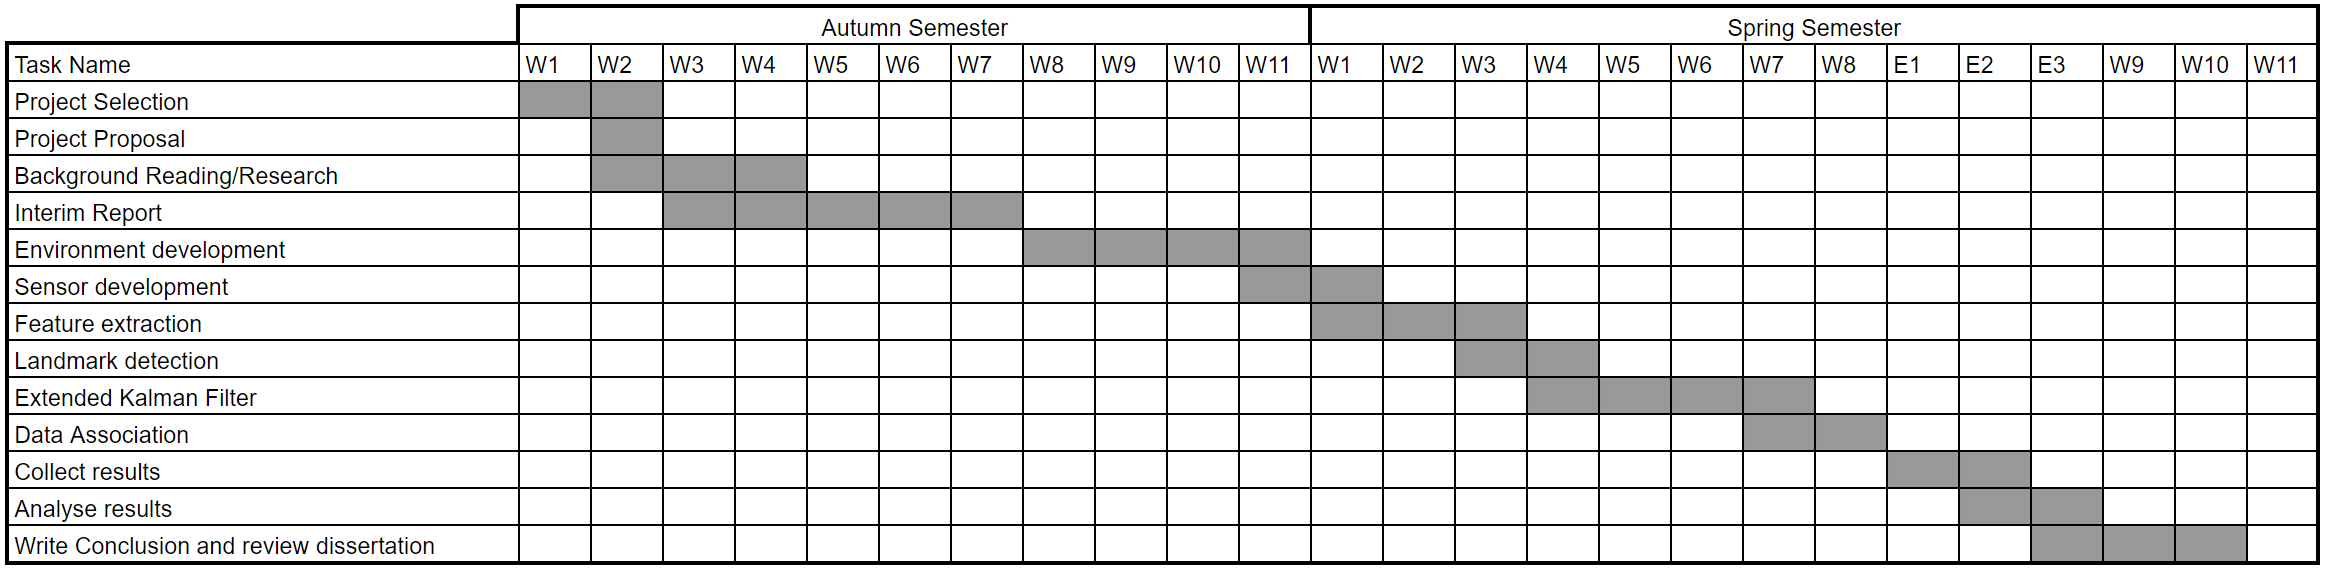
\includegraphics[width=0.8\linewidth]{gantt_chart.png}
    \caption{Gantt chart showing the project plan}
    \label{fig:gantt_chart}
\end{figure}
The execution of my project will be split into various phases, where each phase will focus on an area of development. The
majority of the project will be software development, therefore I have chosen to split this process into various stages. Figure
\ref{fig:gantt_chart} shows the project plan, where the grey bars represent the time spent at each phase. Should my project
overrun, I will have contingency time built into both the Christmas break and the Easter break, which is currently unaccounted
for in the project plan.\\

\subsection{Phase 1 - Research and Planning}
The first phase of my project involves researching and planning. During this period I will create a project proposal,
research SLAM and swarm algorithms, and write this interim report. This phase will be completed by week 7. It is important
to carry out this phase as it provides structure for the whole project, which will help ensure that the project is completed
on time.
\subsection{Phase 2 - Single SLAM Agent}

\begin{figure}[h]
    \centering
    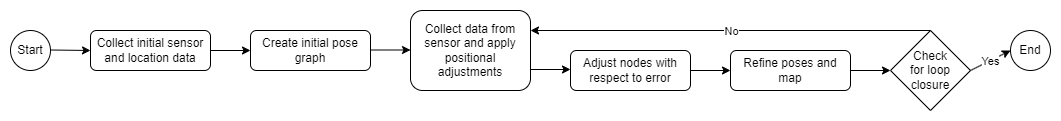
\includegraphics[width=1\linewidth]{flowchart.png}
    \caption{A flow chart of the Pose Graph SLAM algorithm}
    \label{fig:flowchart}
\end{figure}

The second phase of my project is where development will start. I will start by creating a basic simulation environment, where
the user can see the agent and the environment. After, I will implement the Pose Graph SLAM algorithm seen in Figure \ref{fig:flowchart},
on a single agent system. This will give me the experience of implementing SLAM, which will be useful when implementing swarm
algorithms as a good portion of the code will be reusable. This phase will be completed by week 8, and will allow me to follow
on to multi-agent random walks.

\subsection{Phase 3 - Multi-agent Random Walk}
In the third phase, I will implement a multi-agent random walk algorithm. This will allow me to explore the challenges of swarm
communication and agent coordination. I plan to implement the Brownian motion algorithm as a starting point, then if time permits,
I will explore other algorithms, such as Ballistic motion and Levy walk. I will complete this phase by week 11, which will allow me
plenty of time to implement the more complex swarm algorithms.
\subsection{Phase 4 - Centralised Multi-agent SLAM}
The fourth phase will consist of implementing a centralised multi-agent SLAM algorithm. This will finally allow me to combine
the knowledge I would've gained from the previous phases and apply it to a more complex problem. I will look to implement an
algorithm like the multi agent map merging algorithm, which will allow me to combine the maps of single SLAM agents. Furthermore,
I will bring in the communication system developed in Phase 3, which will help structure the agents. This phase will be completed by
week 2 of the Spring semester.
\subsection{Phase 5 - Decentralised Multi-agent SLAM}
The fifth and final phase of development will see me implement a decentralised multi-agent SLAM algorithm. This will be the most
complex phase of development, as it will require me me to combine the SLAM elements of the previous phase with the communication
from Phase 3. I will look to implement an algorithm like C-SLAM (Collaborative Simultaneous Localization And Mapping) \cite{C-SLAM}, and will analyse it's performance and how it scales. This phase
will be completed by week 5 of the Spring semester.
\subsection{Phase 6 - Analysis and Conclusion}
The final phase of my project will largely consist of writing up my findings and analysing the performance of the algorithms. I will
write up my final dissertation, along with creating a poster for the event. I may also spend some time creating visual representations
of my findings, such as graphs and charts. This phase may begin as early as week 4 of the Spring semester and will be completed by
week 10.
\section{Supervisor Meetings}
\subsection{Meeting 1 - 11/10/2023}
Discussed on the project idea and potential directions to take. Discussed the possibility of implementing physical agents,
challenges that may occur and potential ways of implementing swarm algorithms. Need to focus on researching SLAM and swarm
and looking into existing resources.
\subsection{Meeting 2 - 27/10/2023}
Discussed potential algorithms, such as particle filters and graph-based SLAM. We also discussed the logistics of the project,
ensuring that it remains both realistic and achievable. We also discussed the possibility of implementing physical agents,
and where relevant resources could be found.
\subsection{Meeting 3 - 14/11/2023}
Started with feedback on the interim report - discussing the structure and content. After we discussed how the project will
move forward and the next steps to take. Given the interim report is now complete, we can focus mainly on development, following
the project plan. As I have already developed a basic simulation interface, I can now move onto implementing my first SLAM algorithm.
\subsection{Meeting 4 - 08/12/2023}
In this meeting, we turned to ironing out the specifics of the implementation - including looking at existing resources, like
Enki, and concepts that need to be considered, such as Differential Turning. The goal of this meeting was to guide me into
starting to create my environment and first SLAM algorithm, which will be implemented over the christmas break.
\subsection{Meeting 5 - 02/02/2024}
We firstly caught up on progress made over the christmas break. After, we started to look forward to the next steps of the project,
discussing the projects overall direction and the next steps to take. One notable suggestion was the move away from swarm algorithms
and perhaps the move towards multi-agent SLAM, as this would be more achievable in the time frame. Finally, we discussed how I
should manage my time towards the end of the project and how I could start working on my dissertation.
\subsection{Meeting 6 - 09/02/2024}
Started with me demonstrating my current progress, with my environment working, LIDAR sensor appropriately implemented and
my work-in-progress feature detection. We discussed then how I could approach landmark detection and how I planned on implementing
it. We ended the meeting with clearing up questions regarding the project presentation, poster competition and submission.
\subsection{Meeting 7 - 16/02/2024}


%Appendix
\section{Appendices}

\subsection{Project Proposal}
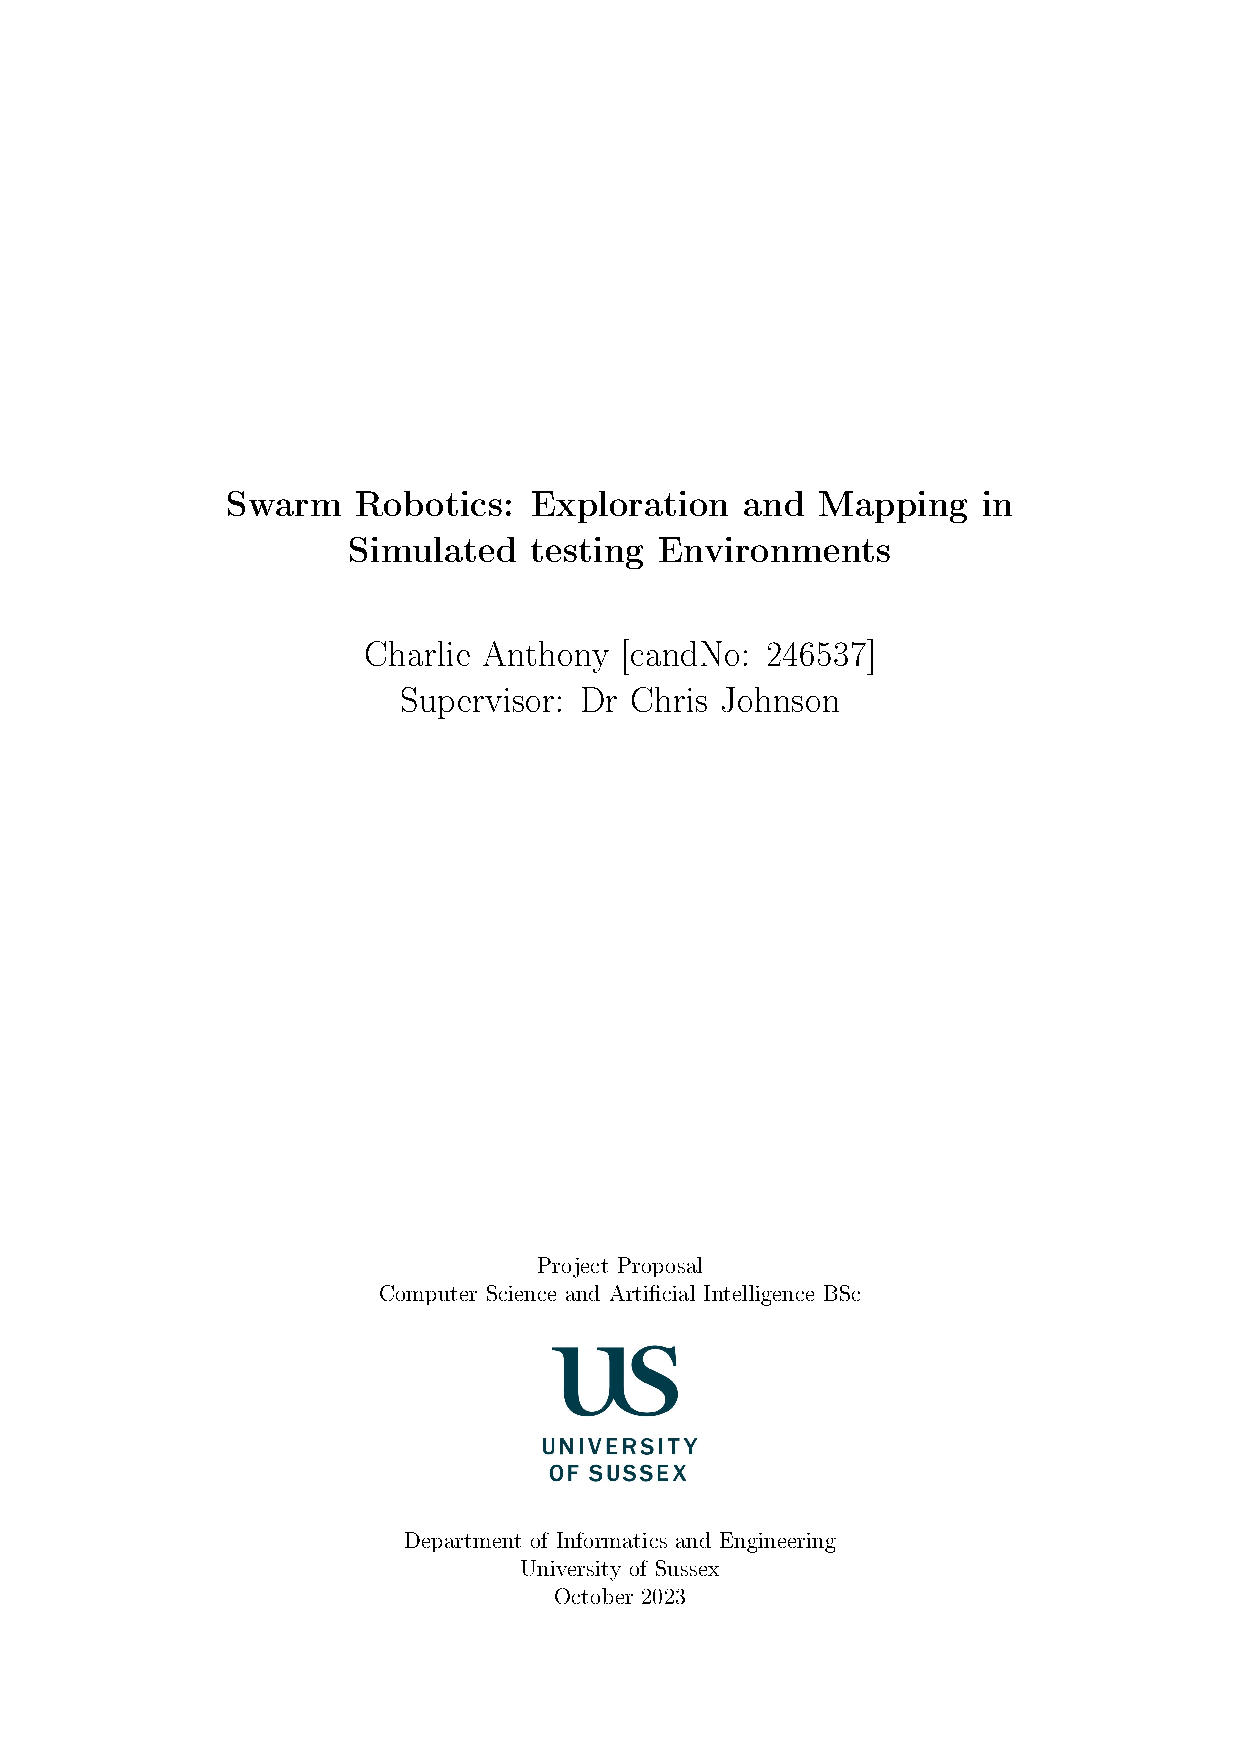
\includepdf[pages=-]{ProjectProposal.pdf}

%References
\section{References}

\begin{thebibliography}{9}

    \bibitem{starling_swarm}
    H. Hildenbrandt, C. Carere, C.K. Hemelrijk
    \textit{Self-organized aerial displays of thousands of starlings: a model}
    \href{https://doi.org/10.1093/beheco/arq149}{https://doi.org/10.1093/beheco/arq149}

    \bibitem{SLAM_overview}
    U. Frese, R. Wagner, T. Röfer
    \textit{A SLAM overview from a users perspective, 2010}
    \href{http://dx.doi.org/10.1007/s13218-010-0040-4}{http://dx.doi.org/10.1007/s13218-010-0040-4}

    \bibitem{intro_to_swarm}
    I. Navarro, F. Matía
    \textit{An Introduction to Swarm Robotics, 2013}
    \href{https://doi.org/10.5402/2013/608164}{https://doi.org/10.5402/2013/608164}

    \bibitem{swarm_SLAM}
    K. Miquel, G. Giorgio, B. Mauro
    \textit{Swarm SLAM: Challenges and Perspectives, 2021}
    \href{https://doi.org/10.3389/frobt.2021.618268}{https://doi.org/10.3389/frobt.2021.618268}

    \bibitem{swarm_random_walks}
    M. Kegeleirs, D. Garzón Ramos,  M. Birattari
    \textit{Random walk exploration for swarm mapping, 2019}
    \href{https://doi.org/10.1007/978-3-030-25332-5_50}{https://doi.org/10.1007/978-3-030-25332-5_50}

    \bibitem{brownian_motion}
    E. Khmelnitsky
    \textit{Brownian Motion and Swarm Dynamics. In Autonomous Mobile Robots and Multi-Robot Systems, 2019}
    \href{https://doi.org/10.1002/9781119213154.ch12}{https://doi.org/10.1002/9781119213154.ch12}

    \bibitem{C-SLAM}
    P. Lajoie, G. Beltrame
    \textit{Swarm-SLAM : Sparse Decentralized Collaborative Simultaneous Localization and Mapping Framework for Multi-Robot Systems, 2023}
    \href{https://doi.org/10.48550/arXiv.2301.06230}{https://doi.org/10.48550/arXiv.2301.06230}

\end{thebibliography}



\end{document}


